\documentclass[]{beamer}


%\usetheme{Darmstadt}
 
\usepackage[T1]{fontenc}
\usepackage[utf8]{inputenc}
\usepackage{url}

\usepackage{amsmath, amssymb}
%\usepackage{varwidth}% http://ctan.org/pkg/varwidth
\usepackage{amsmath}
\usepackage{mathtools}
\usepackage{tikz}

\usepackage{breqn}

\usetikzlibrary{calc,tikzmark,arrows,shapes,backgrounds}
%\usetikzlibrary{positioning, fit, arrows.meta, shapes}
\usetikzlibrary{fit, arrows.meta, shapes}

% used to avoid putting the same thing several times...
% Command \empt{var1}{var2}
%\newcommand{\empt}[2]{$#1^{\langle #2 \rangle}$}
\newcommand{\empt}[2]{$#1^{( #2 )}$}



\setbeamertemplate{footline}[frame number]
%%\setbeamertemplate{headline}{Magister en estadística - PUCV}
 

\usetikzlibrary{arrows.meta}



\title{Modelos Lineales para Clasificación}
\subtitle{Modelo logístico para datos binarios}
\author{Juan Zamora O.}
%\institute{Pontificia Universidad Católica de Valparaíso}
\date{}


%%% LOGO DE LA PAGINA INICIAL
\titlegraphic{
	\begin{tikzpicture}[overlay,remember picture]
		\node[opacity=0.8,below=0.3cm] at (current page.center){		
    			
\includegraphics[width=4cm]{logo_ies}
		};
	\end{tikzpicture}
}
%%% END OF LOGO




%%% LOGO DE CADA LAMINA
\logo{
	\begin{tikzpicture}[overlay,remember picture]
		\node[opacity=0.4,right=1.2cm, above=0.12cm] at (current page.south west){		
    			
\includegraphics[width=2cm]{logo_ies}
		};
	\end{tikzpicture}
}
%%% END OF LOGO



\begin{document}

\begin{frame}[noframenumbering,plain]
    \titlepage
\end{frame}

\section{Intro}
\begin{frame}{Regresión categórica}

    Regresión con datos categóricos persigue el mismo objetivo la regresión 
    sobre variable continua
    \vspace{10pt}

    Representar el enlace entre covariables o variables independientes y una 
    respuesta o variable dependiente
    \vspace{10pt}

    La diferencia más crucial radica en la distribución de la variable dependiente
    y en la función que vincula las covariables con el valor medio de la respuesta\\~\


\end{frame}

\begin{frame}{El caso binario}
    La distribución de la variable dependiente es distinta al caso clásico, debido a que ya
    no será posible poder observar cualquier valor\\~\
    
    En particular, la variable dependiente podrá tomar valores en $\{0,1\}$\\~\

    Sea la variable dependiente codificada por $y=1$ e $y=0$ para indicar la ocurrencia
    o ausencia de un evento\\~\ 

    \begin{tikzpicture}[remember picture, overlay]
        \node[above=1.8cm, left=-1cm] at (current page.south) 
        {
            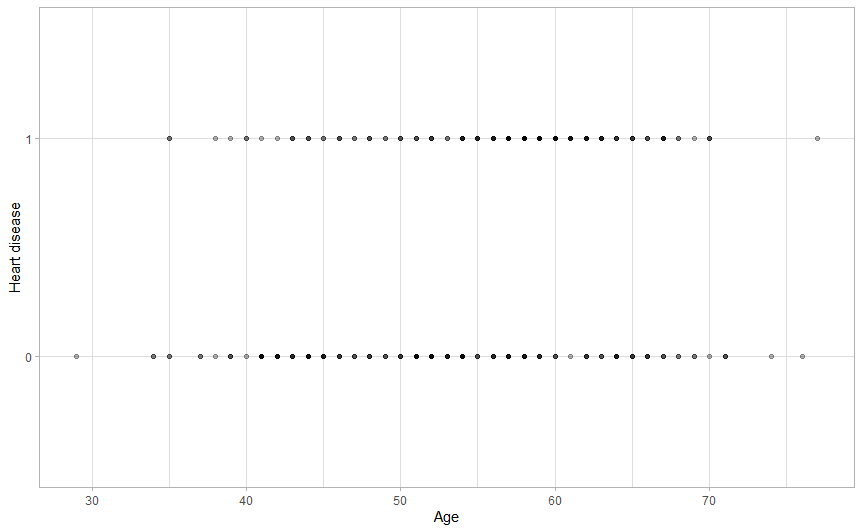
\includegraphics[width=0.5\textwidth]{binary_outcomes.png}
        };
        %\node[below=-1cm,font=\fontsize{5pt}{5pt}\selectfont] at (current page.south)  {Extracted from \url{https://web.stanford.edu/class/cs224n/}};
    \end{tikzpicture}



\end{frame}

\begin{frame}
    \frametitle{}
    La distribución de la variable aleatoria binaria $y\in\{0,1\}$ es caracterizada por 
    la probabilidad $\pi=P(y=1)$\\~\ 
    
    Siendo $P(y=0)=1-\pi $, el valor medio de $y$ se calcula mediante $E[y]=1\times \pi + 0\times (1-\pi )=\pi $\\~\ 

    La varianza es calculada siguiendo el mismo esquema, es decir  
    $$Var[y]=E[y-E[y]]^2=(1-\pi)^2\pi +(0-\pi)^2(1-\pi)^2=\pi (1-\pi)$$

\end{frame}

\begin{frame}
    \frametitle{Odds, Logits y Odds Ratios}

    A menudo se consideran algunas transformaciones de $\pi$ como indicadores del 
    comportamiento aleatorio de la respuesta\\~\ 

    Una medida que compara las probabilidades de ocurrencia y no ocurrencia del evento 
    es los \textbf{Odds} y se define como $$\gamma(\pi)=\frac{P(y=1)}{P(y=0)}=\frac{\pi}{1-\pi }$$

    Alternativamente, también se usa el log de Odds y se denomina función \textbf{logit},
    $$logit\left(\pi \right)=log(\gamma(\pi))$$

\end{frame}

\begin{frame}{Odds, Logits y Odds Ratios}{Comparando dos grupos}
    
    Estas medidas cobran importancia si queremos comparar dos grupos, por ejemplo uno
    experimental y otro de control \\~\ 
    
    Luego, tenemos probabilidades $P(y=1|G=1)$ y $P(y=1|G=2)$, las cuales podemos contrastar
    mediante diferencias $\pi_1-\pi_2$, proporciones $\frac{\pi_1}{\pi_2}$ entre otras \\~\ 
    
    Una medida muy útil son los \textbf{Odds Ratio}, ya que comparan Odds en lugar de 
    probablidades mediante  $\frac{\pi_1/(1-\pi_1)}{\pi_2/(1-\pi_2)}$ \\~\  
    
    Alternativamente, también se usa la transformación
    logaritmica, ya que permite fijar con valor $0$ cuando ambos grupos son equivalentes  
    
    %% despuespodria colocar un ejemplo corto con dos grupos de poblaciones que pueden contagiarse.
\end{frame}

\begin{frame}
    \frametitle{El modelo Logit}

    Cuando existen 2 grupos se usa solo un predictor binario del tipo
    $$logit(\pi(\mathbf{x}))=\mathbf{x}^T\beta $$
    
    Equivalentemente     
    $$\pi(\mathbf{x})=\frac{\exp (\mathbf{x}^T\beta)}{1+\exp(\mathbf{x}^T\beta)}$$

    o en término de Odds
    $$\frac{\pi(x)}{1-\pi(x)}=\exp(\beta_0+\mathbf{x}^T\beta)=\exp(\beta_0)\exp(\mathbf{x}^T\beta)$$

    %Donde $$\beta_0=logit(\pi_2(\mathbf{x}))\ , \ \beta=log\left(\frac{\pi_1(\mathbf{x})/(1-\pi_1(\mathbf{x}))}{\pi_2(\mathbf{x})/(1-\pi_2(\mathbf{x}))}\right)$$

\end{frame}


\begin{frame}{El modelo Logit}{Entendiendo los parámetros}

    Cuando consideramos un modelo lineal $y=\mathbf{x}^T\beta$, el parámetro $\beta$ 
    denota el cambio del valor medio de la respuesta cuando $\mathbf{x}$ aumenta en 
    una unidad\\~\  

    Para el modelo logit, se aplica la misma idea, pero en terminos de logits.
    $$\beta = logit(\pi(x+1)) - logit(\pi(x))$$

\end{frame}

\begin{frame}{El modelo Logit}{Entendiendo los parámetros}
    Desde las perspectiva de las Odds, $\exp(\beta_0)$ representa las Odds cuando $x=0$. Además, estas 
    \textit{cambian} con un factor $\exp(\beta)$ cuando $x$ aumenta en una unidad.\\~\ 

    Entonces esta razón de cambio se puede definir en términos de Odds Ratios 
    $$\exp(\beta)=\dfrac{\pi(x+1)/(1-\pi(x+1))}{\pi(x)/(1-\pi(x))}=\frac{\gamma(\pi(x+1))}{\gamma(\pi(x)    )}$$

    La interpretación de $\beta$ o $\exp(\beta )$ es simple, debido a que modelo logit 
    \textbf{supone} que estos Odds Ratios no dependen de $x$
\end{frame}


\begin{frame}{El modelo Logit}{Caso multivariado}
    Anteriormente, se ha usado $\mathbf{x}$ como un valor escalar. Al existir $m$ covariables continuas,
    el predictor tendrá la forma 
    $$logit(\pi(\mathbf{x})) = \beta_0+x_1\beta_1+x_2\beta_2+\ldots +x_m\beta_m$$

    o bien en términos de Odds
    $$\gamma(\pi(\mathbf{x})) = \exp(\beta_0)\exp(x_1\beta_1)\exp(x_2\beta_2)\ldots \exp(x_m\beta_m)$$

    El análisis del cambio de logits o de Odds es idéntico.  Es decir, $\exp(\beta_j)$ corresponde al \textit{cambio multiplicativo}
    en Odds cuando $x_j$ aumenta en una unidad y todos los demás valores \textbf{permanecen fijos}
\end{frame}

\begin{frame}
    \frametitle{Modelo Logit con predictores binarios}

    Consideremos el caso en que la variable dependiente depende de una sola covariable $x$ que puede tener 
    solo dos valores posibles. Codifiquemos esta covaraible en $\{0,1\}$\\~\  

    La representación habitual será mediante una tabla de contingencia de $2\times 2$\\~\   

    Considerando $\pi(x)=P(y=1|x)$, el modelo logit será entonces
    $$log\left( \frac{\pi(x)}{1-\pi(x)}\right)=\beta_0+x\beta$$
    

\end{frame}

\begin{frame}
    \frametitle{}
    Los Log-Odds en la categoría de referencia ($x=0$)
    $$\beta_0=log\left( \frac{\pi(x=0)}{1-\pi(x=0)}\right)$$

    Por lo tanto, a partir del modelo logit especificado en la lámina anterior,
    $$\beta = log\left( \frac{\pi(x)}{1-\pi(x)}\right) - log\left( \frac{\pi(x=0)}{1-\pi(x=0)}\right)$$
    
    que corresponde al factor en que cambian los logits cuando $x=0$ es reemplazado por $x=1$.
\end{frame}

\begin{frame}
    \frametitle{Modelo Logit con predictores categóricos}

    Como caso más general, también podemos usara covariables que tengan más de 2 valores posibles.\\~\   

    Consideremos una covariable o factor con categorías $\{1,2,\ldots ,  K\}$. La forma general del 
    modelo logit estará dada por 
    $$log\left(\frac{\pi(x=i)}{1-\pi(x=i)}\right)=\beta_0+\beta_i$$

    Si definimos la categoría $K$ como referencia, entonces $\beta_0 =log \left(\frac{\pi(x=K)}{1-\pi(x=K)}\right)$\\~\ 

\end{frame}

\begin{frame}
    Luego, cambio aditivo en logit si la categoría de referencia $K$ es reemplazada por la $i$, estará dado por 
    $$\beta_i=log\left( \frac{\pi(x=i)}{1-\pi(x=i)}\right) - log\left( \frac{\pi(x=K)}{1-\pi(x=K)}\right)$$

    Alternativamente (también para el caso binario), siempre podemos considerar las versiones exponencial 
    $$\exp(\beta_0)=\frac{\pi(x=K)}{1-\pi(x=K)}$$

    $$exp(\beta_i)=\exp\left[log\left( \frac{\pi(x=i)}{1-\pi(x=i)}\right) - log\left( \frac{\pi(x=K)}{1-\pi(x=K)}\right)\right]$$


\end{frame}

\begin{frame}
    \frametitle{Estimación de los parámetros}

    Considerando $n$ observaciones independientes $(x_i,y_i)_{i=1}^{n}$ con $y_i\in\{0,1\}$, para el modelo lineal logit 
     $$P(y_i=1|x_i)=\frac{\exp(\mathbf{x}^T\beta )}{1+\exp(\mathbf{x}^T\beta )}$$

    los parámetros a estimar son los coeficientes de regresión $\mathbf{\beta}$\\~\  

    Para esto el método más usado es \textbf{Máxima Verosimilitud}. 

\end{frame}

\begin{frame}{Estimación de los parámetros}{Máxima Verosimilitud}
    Primero se construye la Verosimilitud de los parámetros desconocidos para los datos observados.\\~\   
    
    Esta Verosimilitud representa la probabilidad de observar la muestra de los datos en función 
    de los parámetros desconocidos
    $$\mathsf{L}(\beta)=\prod_{i=1}^{n}\pi(x_i)^{y_i}(1-\pi(x_i))^{1-y_i}$$

    Notar que $\pi(x_i)^{y_i}(1-\pi(x_i))^{1-y_i}$ simplifica a $\pi(x_i)$ cuando $y_i=1$ y a 
    $(1-\pi(x_i))$ cuando $y_i=0$. Además se usa el producto, debido a que $y_,\ldots ,y_n$ dado 
    $x_1,\ldots , x_n$ son considerados como independientes

\end{frame}

\begin{frame}{Estimación de los parámetros}{Máxima Verosimilitud}
    El objetivo de MV es encontrar el vector de parámetros $\widehat{\beta}$ que maximiza la 
    Verosimilitud o la Log-Verosimilitud $l(\widehat{\beta})$\\~\  

    Para esto, se resuelve el sistema de ecuaciones generado mediante 
    $$\delta l(\beta)/\delta \beta = (\delta l(\beta)/\delta \beta_1,\delta l(\beta)/\delta \beta_2,\ldots , \delta l(\beta)/\delta \beta_p   )^T=\mathbf{0}$$

    Al calcular las derivadas parciales expresadas anteriormente, este sistema queda expresado como 
    $$\delta l(\beta)/\delta \beta = \sum_{i=1}^{n}\mathbf{x}_i\frac{\delta h(\mathbf{x}_i^T\beta )}{\delta \beta }\frac{(y_i -\pi(\mathbf{x}_i))}{\pi(\mathbf{x}_i)(1-\pi(\mathbf{x}_i))}$$ 

    con $h(x)=\frac{\exp(x)}{1+\exp(x)}$ y $\pi(\mathbf{x}_i)=h(\mathbf{x}_i^T\beta )$
\end{frame}

\begin{frame}{Estimación de los parámetros}{Máxima Verosimilitud}
    Para el modelo logit se obtiene 
    $$\frac{\delta l(\beta)}{\delta \beta_j}=\sum_{i=1}^n x_{ij}(y_i-\pi(x_i))$$

    El sistema resultante se resuelve posteriormente de manera iterativa.
\end{frame}

\begin{frame}
    \frametitle{Medición de la calidad del ajuste}

    Previo al uso de un modelo ajustado para  inferencia es importante verificar la calidad del ajuste.
    Es decir, medir el grado de discrepancia entre el modelo ajustado y las observaciones.\\~\  

    La suma de residuos al cuadrado usada para la regresión es inapropiada cuando la respuesta es binaria.\\~\  

    La \textit{Deviance} permite comparar entre el ajuste obtenido y un ajuste ideal.
    $$2\{l(\mbox{Modelo saturado})-l(\mbox{Modelo ajustado})\}$$



\end{frame}
%%%%%%%%%%%%%%%%
\end{document}